\documentclass[twoside]{book}

% Packages required by doxygen
\usepackage{fixltx2e}
\usepackage{calc}
\usepackage{doxygen}
\usepackage[export]{adjustbox} % also loads graphicx
\usepackage{graphicx}
\usepackage[utf8]{inputenc}
\usepackage{makeidx}
\usepackage{multicol}
\usepackage{multirow}
\PassOptionsToPackage{warn}{textcomp}
\usepackage{textcomp}
\usepackage[nointegrals]{wasysym}
\usepackage[table]{xcolor}

% Font selection
\usepackage[T1]{fontenc}
\usepackage[scaled=.90]{helvet}
\usepackage{courier}
\usepackage{amssymb}
\usepackage{sectsty}
\renewcommand{\familydefault}{\sfdefault}
\allsectionsfont{%
  \fontseries{bc}\selectfont%
  \color{darkgray}%
}
\renewcommand{\DoxyLabelFont}{%
  \fontseries{bc}\selectfont%
  \color{darkgray}%
}
\newcommand{\+}{\discretionary{\mbox{\scriptsize$\hookleftarrow$}}{}{}}

% Page & text layout
\usepackage{geometry}
\geometry{%
  a4paper,%
  top=2.5cm,%
  bottom=2.5cm,%
  left=2.5cm,%
  right=2.5cm%
}
\tolerance=750
\hfuzz=15pt
\hbadness=750
\setlength{\emergencystretch}{15pt}
\setlength{\parindent}{0cm}
\setlength{\parskip}{3ex plus 2ex minus 2ex}
\makeatletter
\renewcommand{\paragraph}{%
  \@startsection{paragraph}{4}{0ex}{-1.0ex}{1.0ex}{%
    \normalfont\normalsize\bfseries\SS@parafont%
  }%
}
\renewcommand{\subparagraph}{%
  \@startsection{subparagraph}{5}{0ex}{-1.0ex}{1.0ex}{%
    \normalfont\normalsize\bfseries\SS@subparafont%
  }%
}
\makeatother

% Headers & footers
\usepackage{fancyhdr}
\pagestyle{fancyplain}
\fancyhead[LE]{\fancyplain{}{\bfseries\thepage}}
\fancyhead[CE]{\fancyplain{}{}}
\fancyhead[RE]{\fancyplain{}{\bfseries\leftmark}}
\fancyhead[LO]{\fancyplain{}{\bfseries\rightmark}}
\fancyhead[CO]{\fancyplain{}{}}
\fancyhead[RO]{\fancyplain{}{\bfseries\thepage}}
\fancyfoot[LE]{\fancyplain{}{}}
\fancyfoot[CE]{\fancyplain{}{}}
\fancyfoot[RE]{\fancyplain{}{\bfseries\scriptsize Generated by Doxygen }}
\fancyfoot[LO]{\fancyplain{}{\bfseries\scriptsize Generated by Doxygen }}
\fancyfoot[CO]{\fancyplain{}{}}
\fancyfoot[RO]{\fancyplain{}{}}
\renewcommand{\footrulewidth}{0.4pt}
\renewcommand{\chaptermark}[1]{%
  \markboth{#1}{}%
}
\renewcommand{\sectionmark}[1]{%
  \markright{\thesection\ #1}%
}

% Indices & bibliography
\usepackage{natbib}
\usepackage[titles]{tocloft}
\setcounter{tocdepth}{3}
\setcounter{secnumdepth}{5}
\makeindex

% Hyperlinks (required, but should be loaded last)
\usepackage{ifpdf}
\ifpdf
  \usepackage[pdftex,pagebackref=true]{hyperref}
\else
  \usepackage[ps2pdf,pagebackref=true]{hyperref}
\fi
\hypersetup{%
  colorlinks=true,%
  linkcolor=blue,%
  citecolor=blue,%
  unicode%
}

% Custom commands
\newcommand{\clearemptydoublepage}{%
  \newpage{\pagestyle{empty}\cleardoublepage}%
}

\usepackage{caption}
\captionsetup{labelsep=space,justification=centering,font={bf},singlelinecheck=off,skip=4pt,position=top}

%===== C O N T E N T S =====

\begin{document}

% Titlepage & ToC
\hypersetup{pageanchor=false,
             bookmarksnumbered=true,
             pdfencoding=unicode
            }
\pagenumbering{alph}
\begin{titlepage}
\vspace*{7cm}
\begin{center}%
{\Large My Project }\\
\vspace*{1cm}
{\large Generated by Doxygen 1.8.13}\\
\end{center}
\end{titlepage}
\clearemptydoublepage
\pagenumbering{roman}
\tableofcontents
\clearemptydoublepage
\pagenumbering{arabic}
\hypersetup{pageanchor=true}

%--- Begin generated contents ---
\chapter{flea\+Market小型二手交易平台}
\label{md_README}
\Hypertarget{md_README}
\subsection*{一个运行在\+Linux系统上的小型web服务器。}


\begin{DoxyItemize}
\item 纯\+C++开发,未使用任何web框架
\item 采用epoll,能承受校内ip的高并发访问
\item 利用json进行前后端数据的传输,支持传输图片
\item 使用mysql数据库保存用户与商品信息
\item 前端开发使用了bootscrap+j\+Query框架 (注:后端代码在back\+End分支内) 
\end{DoxyItemize}
\chapter{Hierarchical Index}
\section{Class Hierarchy}
This inheritance list is sorted roughly, but not completely, alphabetically\+:\begin{DoxyCompactList}
\item \contentsline{section}{e\+Poll\+Monitor}{\pageref{classePollMonitor}}{}
\item \contentsline{section}{Mysql}{\pageref{classMysql}}{}
\item \contentsline{section}{Socket}{\pageref{classSocket}}{}
\begin{DoxyCompactList}
\item \contentsline{section}{Connect\+Socket}{\pageref{classConnectSocket}}{}
\item \contentsline{section}{Listen\+Socket}{\pageref{classListenSocket}}{}
\end{DoxyCompactList}
\end{DoxyCompactList}

\chapter{Class Index}
\section{Class List}
Here are the classes, structs, unions and interfaces with brief descriptions\+:\begin{DoxyCompactList}
\item\contentsline{section}{\hyperlink{classConnectSocket}{Connect\+Socket} }{\pageref{classConnectSocket}}{}
\item\contentsline{section}{\hyperlink{classePollMonitor}{e\+Poll\+Monitor} }{\pageref{classePollMonitor}}{}
\item\contentsline{section}{\hyperlink{classListenSocket}{Listen\+Socket} }{\pageref{classListenSocket}}{}
\item\contentsline{section}{\hyperlink{classMysql}{Mysql} }{\pageref{classMysql}}{}
\item\contentsline{section}{\hyperlink{classSocket}{Socket} }{\pageref{classSocket}}{}
\end{DoxyCompactList}

\chapter{Class Documentation}
\hypertarget{classConnectSocket}{}\section{Connect\+Socket Class Reference}
\label{classConnectSocket}\index{Connect\+Socket@{Connect\+Socket}}


Inheritance diagram for Connect\+Socket\+:\nopagebreak
\begin{figure}[H]
\begin{center}
\leavevmode
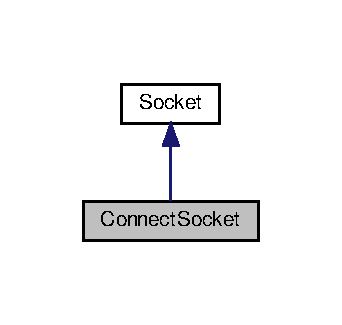
\includegraphics[width=164pt]{classConnectSocket__inherit__graph}
\end{center}
\end{figure}


Collaboration diagram for Connect\+Socket\+:\nopagebreak
\begin{figure}[H]
\begin{center}
\leavevmode
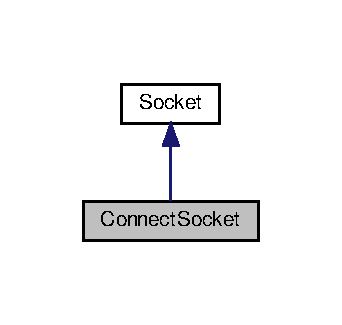
\includegraphics[width=164pt]{classConnectSocket__coll__graph}
\end{center}
\end{figure}
\subsection*{Public Member Functions}
\begin{DoxyCompactItemize}
\item 
\mbox{\Hypertarget{classConnectSocket_ad1db4adc587e2b582d42e71009dd3d6e}\label{classConnectSocket_ad1db4adc587e2b582d42e71009dd3d6e}} 
{\bfseries Connect\+Socket} (\hyperlink{classListenSocket}{Listen\+Socket} $\ast$\&p\+Server)
\item 
\mbox{\Hypertarget{classConnectSocket_a39263b739672a96ad911ff57803ce9d7}\label{classConnectSocket_a39263b739672a96ad911ff57803ce9d7}} 
std\+::string {\bfseries receive} ()
\item 
\mbox{\Hypertarget{classConnectSocket_ae3792d4b1c27f814c97ba06c15dc323a}\label{classConnectSocket_ae3792d4b1c27f814c97ba06c15dc323a}} 
void {\bfseries send} (const std\+::string \&message)
\end{DoxyCompactItemize}
\subsection*{Additional Inherited Members}


The documentation for this class was generated from the following file\+:\begin{DoxyCompactItemize}
\item 
mysocket.\+h\end{DoxyCompactItemize}

\hypertarget{classePollMonitor}{}\section{e\+Poll\+Monitor Class Reference}
\label{classePollMonitor}\index{e\+Poll\+Monitor@{e\+Poll\+Monitor}}
\subsection*{Public Member Functions}
\begin{DoxyCompactItemize}
\item 
\mbox{\Hypertarget{classePollMonitor_aebeaa590ed90cbec989b191f71065416}\label{classePollMonitor_aebeaa590ed90cbec989b191f71065416}} 
void {\bfseries add} (int fd)
\item 
\mbox{\Hypertarget{classePollMonitor_a284229cc3cdf2990f9dc254dd290f1ff}\label{classePollMonitor_a284229cc3cdf2990f9dc254dd290f1ff}} 
void {\bfseries drop} (int index)
\item 
\mbox{\Hypertarget{classePollMonitor_ad9ed7d467f348301e2deed4da9f31e7e}\label{classePollMonitor_ad9ed7d467f348301e2deed4da9f31e7e}} 
int {\bfseries wait} (int timeout)
\end{DoxyCompactItemize}
\subsection*{Public Attributes}
\begin{DoxyCompactItemize}
\item 
\mbox{\Hypertarget{classePollMonitor_aa119e786a1e3bbe7a5f9072a66697bc1}\label{classePollMonitor_aa119e786a1e3bbe7a5f9072a66697bc1}} 
int {\bfseries epfd}
\item 
\mbox{\Hypertarget{classePollMonitor_abc3257cf7ac7a8296497ee7dcf2d11fe}\label{classePollMonitor_abc3257cf7ac7a8296497ee7dcf2d11fe}} 
epoll\+\_\+event {\bfseries Set} \mbox{[}M\+A\+X\+\_\+\+C\+L\+I\+E\+N\+T\+\_\+\+N\+UM\mbox{]} \{\}
\end{DoxyCompactItemize}


The documentation for this class was generated from the following file\+:\begin{DoxyCompactItemize}
\item 
epoll.\+h\end{DoxyCompactItemize}

\hypertarget{classListenSocket}{}\section{Listen\+Socket Class Reference}
\label{classListenSocket}\index{Listen\+Socket@{Listen\+Socket}}


Inheritance diagram for Listen\+Socket\+:\nopagebreak
\begin{figure}[H]
\begin{center}
\leavevmode
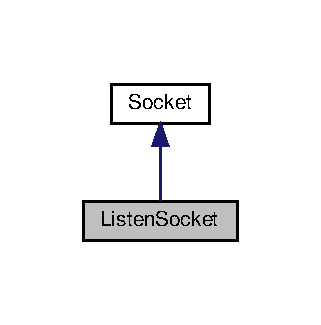
\includegraphics[width=154pt]{classListenSocket__inherit__graph}
\end{center}
\end{figure}


Collaboration diagram for Listen\+Socket\+:\nopagebreak
\begin{figure}[H]
\begin{center}
\leavevmode
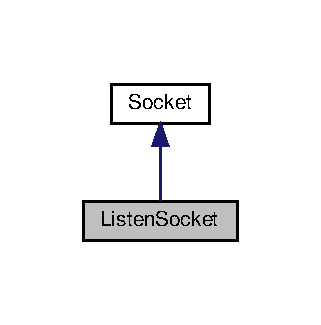
\includegraphics[width=154pt]{classListenSocket__coll__graph}
\end{center}
\end{figure}
\subsection*{Public Member Functions}
\begin{DoxyCompactItemize}
\item 
\mbox{\Hypertarget{classListenSocket_a911d568a28385f01093bfa1c758cf439}\label{classListenSocket_a911d568a28385f01093bfa1c758cf439}} 
{\bfseries Listen\+Socket} (uint32\+\_\+t ip, int port, int listen\+Number)
\end{DoxyCompactItemize}
\subsection*{Additional Inherited Members}


The documentation for this class was generated from the following file\+:\begin{DoxyCompactItemize}
\item 
mysocket.\+h\end{DoxyCompactItemize}

\hypertarget{classMysql}{}\section{Mysql Class Reference}
\label{classMysql}\index{Mysql@{Mysql}}
\subsection*{Public Member Functions}
\begin{DoxyCompactItemize}
\item 
\mbox{\Hypertarget{classMysql_a4ba5ab785eff2f5222f746bbea1d425d}\label{classMysql_a4ba5ab785eff2f5222f746bbea1d425d}} 
bool {\bfseries connect} (const char $\ast$host=\char`\"{}localhost\char`\"{}, const char $\ast$user=\char`\"{}billions\char`\"{}, const char $\ast$password=\char`\"{}123456\char`\"{}, const char $\ast$database=\char`\"{}flea\+Market2\char`\"{})
\item 
\mbox{\Hypertarget{classMysql_a379a7268596be68a18121dfeac3cd097}\label{classMysql_a379a7268596be68a18121dfeac3cd097}} 
bool {\bfseries execute} (const string \&Sql\+Sentence)
\item 
\mbox{\Hypertarget{classMysql_a8ae91a035b0927869ef6a8e64cd893de}\label{classMysql_a8ae91a035b0927869ef6a8e64cd893de}} 
string {\bfseries query} (const string \&Sql\+Sentence)
\end{DoxyCompactItemize}
\subsection*{Public Attributes}
\begin{DoxyCompactItemize}
\item 
\mbox{\Hypertarget{classMysql_aa277c70c117d65e9145ded86a1e6b7e8}\label{classMysql_aa277c70c117d65e9145ded86a1e6b7e8}} 
M\+Y\+S\+QL $\ast$ {\bfseries p}
\end{DoxyCompactItemize}


The documentation for this class was generated from the following file\+:\begin{DoxyCompactItemize}
\item 
mysql.\+h\end{DoxyCompactItemize}

\hypertarget{classSocket}{}\section{Socket Class Reference}
\label{classSocket}\index{Socket@{Socket}}


Inheritance diagram for Socket\+:\nopagebreak
\begin{figure}[H]
\begin{center}
\leavevmode
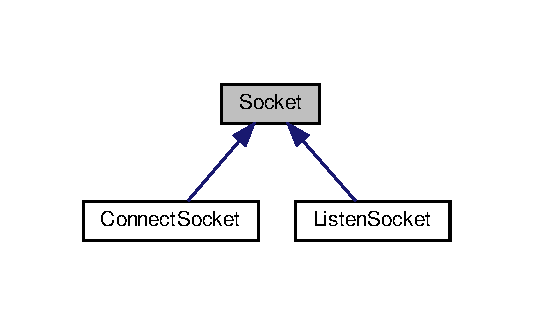
\includegraphics[width=256pt]{classSocket__inherit__graph}
\end{center}
\end{figure}
\subsection*{Public Member Functions}
\begin{DoxyCompactItemize}
\item 
\mbox{\Hypertarget{classSocket_a016ecd3f448e9d0b9cc850e67b69edfd}\label{classSocket_a016ecd3f448e9d0b9cc850e67b69edfd}} 
std\+::string {\bfseries get\+Addr} ()
\end{DoxyCompactItemize}
\subsection*{Public Attributes}
\begin{DoxyCompactItemize}
\item 
\mbox{\Hypertarget{classSocket_a378d057b3f318732cfeec23fce1155ea}\label{classSocket_a378d057b3f318732cfeec23fce1155ea}} 
sockaddr\+\_\+in {\bfseries addr}
\item 
\mbox{\Hypertarget{classSocket_ac7873ea787c01454ce02925367130f23}\label{classSocket_ac7873ea787c01454ce02925367130f23}} 
int {\bfseries fd}
\end{DoxyCompactItemize}


The documentation for this class was generated from the following file\+:\begin{DoxyCompactItemize}
\item 
mysocket.\+h\end{DoxyCompactItemize}

%--- End generated contents ---

% Index
\backmatter
\newpage
\phantomsection
\clearemptydoublepage
\addcontentsline{toc}{chapter}{Index}
\printindex

\end{document}
